\documentclass[a4paper,12pt]{article}
\usepackage[a4paper,top=5cm,bottom=4cm,left=3.6cm,right=3.6cm]{geometry}
\usepackage[T1]{fontenc}
\usepackage[utf8]{inputenc}
\usepackage[english]{babel}
\usepackage{graphicx}
\usepackage{amsmath}
\usepackage{amsfonts}
\usepackage{amsthm}
\usepackage{enumerate}
\usepackage{enumitem}
\usepackage{physics}
\usepackage{bm}
\usepackage{setspace}
\usepackage{caption}
\usepackage{mathtools}

\usepackage[
backend=biber,
style=numeric,
citestyle=numeric,
]{biblatex}
\addbibresource{./report_bib.bib}
\usepackage[autostyle]{csquotes}

\captionsetup{font=footnotesize}


\newtheorem{definition}{Definition}
\newtheorem{prop}{Proposition} 



\begin{document}
	
	%% FRONT PAGE
	\begin{titlepage}
	    \thispagestyle{empty}
	    \newgeometry{left=2cm,right=2cm}
	    \begin{center}
	    	
\includegraphics[width = 4cm]{./polimi-logo.png}\\ \vspace{3mm}
	    	\normalsize{\textsc{Course of Numerical Analysis for Partial Differential Equations}}
	    	
	    	\vspace{20mm}
	    	\rule{15cm}{0.1mm} \\ \vspace{4.5mm}
	    	 \Huge{\textbf{DISCONTINUOUS GALERKIN APPROXIMATION FOR CARDIAC ELECTROPHYSIOLOGY}} \\
	    	\rule{15cm}{0.1mm}
	    	\vspace{20mm}
	    	
	    	\Large{
	    	\begin{align*}
	    	\emph{Authors:}& \hspace{5mm} \textsc{ Federica Botta, Matteo Calafà}\\
	    	\emph{Supervisors:}& \hspace{5mm} \textsc{ Christian Vergara, Paola Antonietti}
	    	\end{align*}
	         } \\
	    	\vspace{35mm}
	    	\large{\textsc{A.Y. 2020/2021}}
	    \end{center}
	\end{titlepage}



    \restoregeometry
    
    %% TABLE OF CONTENTS
    \tableofcontents
    \newpage
    
    %% ABSTRACT
    \section{Introduction}
    \subsection{Abstract}
    The aim of the project is to study and implement a suitable numerical scheme for the resolution of the \emph{Bidomain Problem}, a famous system of equations that has been developed in the context of the electrophysiology of human heart. \\
    This work is basically the continuation of a two-years-long study carried out by three past course projects (\cite{bagnara}, \cite{andreotti}, \cite{marta}). In particular, the very goal of this project is to improve the results obtained in \parencite{marta} (\citeauthor{marta}) for the Bidomain model. In fact, even if a \emph{Discontinuous Galerkin} discretization has been successfully implemented, results are not satisfactory from the point of view of stability and convergence. We think this notice is noteworthy as this work is primarily based on these provided data and codes. Through this article, it will be illustrated how we managed to solve these problems extending, optimizing and correcting these past numerical strategies.
    
    %% PHYSICAL PROBLEM
    \subsection{The physical problem}
    We intend to present the physical meaning of the Bidomain equations very briefly since it has already been widely shown in the previous project (\citeauthor{marta}). For a more complete explanation, we instead refer to \cite{acta}.\\
    The mechanical contraction and expansion of human heart has its origin in the \emph{electrical activation} of the cardiac cells. At every heart-beat, myocyties are activated and deactivated following a characteristic electrical cycle (fig \ref{potential_cycle}). 
    
    
    \begin{figure}[h]
    \begin{center}
    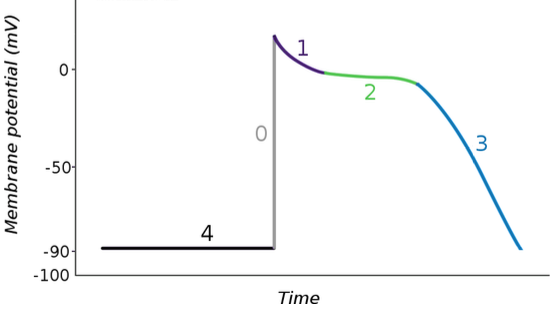
\includegraphics[width = 7cm]{./potential_cycle.png}
    \caption{Membrane potential in function of time (one cardiac cycle)}
    \label{potential_cycle}
    \end{center}
    \end{figure}
    
    \noindent The cell is initially at rest ($-90mV$, step 4). At a certain point, its potential increases rapidly ($\approx2ms$) and reaches the value of $+20mV$: the cell is activated. Later, a plateau near $0mV$ is observed and then a slow repolarization to the initial potential. \\
    From a microscopical point of view, we could study the dynamics acting in each single cell (as a consequence of the passage of chemical ions through specific channels, e.g. $Ca2+,Na+,K+$). From a macroscopical point of view, instead, one can think about it as a continuous electrical diffusion over the entire cardiac surface. Even if this consists in a very rapid phenomenon, the study of such propagation could be very interesting in order, for instance, to detect diseases in sick patients.
    
    \subsection{Mathematical models}
    Starting from the circuit in figure \ref{electrical_circuit}, applying some general electromagnetism laws and some calculations, the Bidomain model has been formulated (see \parencite{acta} for more details and/or \parencite{colli_franzone} for the complete passages).
    
    \begin{figure}[h]
    	\begin{center}
    		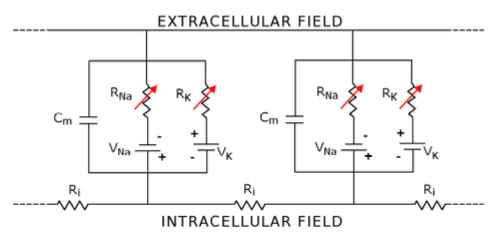
\includegraphics[width = 7cm]{./electrical_circuit.png}
    		\caption{Simplified circuit to model the intracellular and extracellular potentials dynamics}
    		\label{electrical_circuit}
    	\end{center}
    \end{figure}
    
    \noindent The general formulation is then: \vspace{3mm}
    \begin{definition}[Bidomain model]
	\begin{equation*}
	\begin{cases}
	\chi_m C_m\pdv{V_m}{t} - \nabla \cdot (\Sigma_i \nabla \phi_i) + \chi_m I_{ion} = I_i^{ext}    & \text{in } \Omega_{mus} \cross (0,T]
	\\
	-\chi_m C_m\pdv{V_m}{t} - \nabla \cdot (\Sigma_e \nabla \phi_e) - \chi_m I_{ion} = -I_e^{ext}    & \text{in } \Omega_{mus} \cross (0,T]
	\end{cases}
	\end{equation*}
    \end{definition}
	\vspace{3mm}
	
	where:
	\begin{itemize}[label=\textendash]
		\item $\bm{\phi_i, \phi_e}$ are the \emph{Intracellular and Extracelllular Potentials} (unknowns)
		\item $V_m = \phi_i-\phi_e$ is the \emph{Trans-membrane Potential}
		\item $\chi_m,C_m, \Sigma_i, \Sigma_e$ are known constants
		\item $I_i^{ext},I_e^{ext}$ are applied currents
		\item $I_{ion}$ is the \emph{Ionic Current}
		\item $\Omega_{mus}$ is the cardiac domain (myocardium + endocardium + epicardium)
	\end{itemize}
    
    \vspace{4mm}
    \noindent Actually, this system is not complete since it misses boundary and initial conditions and a suitable model for $I_{ion}$. Initial conditions and Neumann boundary conditions for $\phi_i$ and $\phi_e$ are then imposed. For the definition of $I_{ion}$, instead, a \emph{reduced ionic model} is chosen, in particular the \emph{FitzHugh-Nagumo model}. Summing up:
    
    \begin{definition}[Bidomain + FitzHugh-Nagumo model with Neumann boundary conditions]\label{def1}
    	\begin{equation*}
    	\begin{cases}
    	\chi_m C_m\pdv{V_m}{t} - \nabla \cdot (\Sigma_i \nabla \phi_i) + \chi_m I_{ion}(V_m,w) = I_i^{ext}    & \text{in } \Omega_{mus} \cross (0,T]
    	\\
    	-\chi_m C_m\pdv{V_m}{t} - \nabla \cdot (\Sigma_e \nabla \phi_e) - \chi_m I_{ion}(V_m,w) = -I_e^{ext}    & \text{in } \Omega_{mus} \cross (0,T]
    	\\
    	I_{ion}(V_m,w)=kV_m(V_m-a)(V_m-1)-w & \text{in } \Omega_{mus} \cross (0,T]
    	\\
    	\pdv{w}{t} = \epsilon(V_m-\gamma w)  & \text{in } \Omega_{mus} \cross (0,T]
    	\\
    	\Sigma_i\nabla \phi_i \cdot n = b_i   & \text{on } \partial \Omega_{mus} \cross (0,T]
    	\\
    	\Sigma_e\nabla \phi_e \cdot n = b_e   & \text{on } \partial \Omega_{mus} \cross (0,T]
    	\\
    	\text{Initial conditions for } \phi_i,\phi_e, w & \text{in } \Omega_{mus}\cross\{t=0\}
    	\end{cases}
    	\end{equation*}
    \end{definition}
    \vspace{3mm}
    where:
    \begin{itemize}[label=\textendash]
    	\item $\bm{w}$ is the \emph{gating variable} (unknown)
    	\item $k,a,\epsilon,\gamma$ are known constants
    	\item $b_i,b_e$ are the boundary conditions data
    	\item $n$ is the outward normal vector
    \end{itemize}

    \vspace{4mm}
    \noindent From now on, the system of definition \ref{def1} will be the reference analytical problem for the development of numerical schemes.\\
    To conclude, there exist other famous and useful models, such as the \emph{Monodomain model}. But this is just a simplification of the Bidomain as in this case it is assumed that $\phi_i$ and $\phi_e$ are proportional. However, thanks to its simplicity, we often tested the code starting from the Monodomain implementation of the project \cite{andreotti} instead of analyzing directly the Bidomain.

    \subsection{Formulations}
    \subsubsection{DG discrete formulation}
    We have seen the bidomain model in a complete form in \ref{def1}. We introduce now a triangulation $\tau_h$ over $\Omega$, with $\mathcal{F} _h=\mathcal{F} _h^I \cup \mathcal{F} _h^B$ set of the faces of the elements, which includes the internal and boundary faces respectively, and the DG space $V_h^k = \{v_h \in L^2 : v_h|_\mathcal{K} \in \mathbb{P}^{k}(\mathcal{K})  \quad \forall \mathcal{K} \in \tau_h \}$, where k is the degree of the piecewise continuos polynomial.
    
    We obtain the semi discrete DG formulation:
    \begin{equation*}
    \begin{gathered}
    \text{For any time } t \in [0,T] \text{ find } \Phi_h(t)=[\phi_i^h(t),\phi_e^h(t)]^T \in [V_h^k]^2 \text{ and } \omega_h(t) \in V_h^k:\\
    \sum_{K \in \tau_h} \int_K{ \chi_m C_m \pdv{V_m^h}{t} V_h d\omega}+a_i(\phi_i^h,v_h)+\sum_{K \in \tau_h} \int_K{ \chi_m k (V_m^h-1)(V_m^h-a) V_m^h v_h d\omega}+\\
    +\sum_{K \in \tau_h} \int_K{ \chi_m w_h v_h d\omega}=(I_i^{ext},v_h) \qquad \forall v_h \in V_h^p\\
    \newline
    -\sum_{K \in \tau_h} \int_K{ \chi_m C_m \pdv{V_m^h}{t} V_h d\omega}+a_e(\phi_e^h,v_h)-\sum_{K \in \tau_h} \int_K{ \chi_m k (V_m^h-1)(V_m^h-a) V_m^h v_h d\omega}+\\
    -\sum_{K \in \tau_h} \int_K{ \chi_m w_h v_h d\omega}=(-I_e^{ext},v_h) \qquad \forall v_h \in V_h^p\\
    \newline
    \sum_{K \in \tau_h} \int_K{\pdv{w_h}{t}v_h d\omega}=\sum_{k \in \tau_h} \int_K{\epsilon (V_m^h-\gamma w_h) v_h d\omega} \qquad \forall v_h \in V_h^p\\
    \end{gathered}
    \end{equation*}
    where:
    \begin{equation*}
    \begin{gathered}
    a_k(\phi_k^h,v_h)=\sum_{K \in \tau_h} \int_K{(\Sigma_k \nabla_h \phi_k^h) \cdot \nabla_h v_h d\omega}-\sum_{F \in \mathcal{F}_h^I} \int_F { \{\{\Sigma_k \nabla_h \phi_k^h \}\} \cdot [[v_h]] d\sigma}+\\
    -\delta \sum_{F \in \mathcal{F}_h^I} \int_F{ \{\{\Sigma_k \nabla_h v_h\}\} \cdot [[\phi_k^h]]d\sigma}+\sum_{F \in \mathcal{F}_h^I}\int_F {\gamma [[\phi_k^h]] \cdot [[v_h]] d\sigma} \qquad \text{for k=i,e}\\
    \newline
    (I_i^{ext},v_h)=\sum_{K \in \tau_h} \int_K {I_i^{ext} v_h d\omega}+\int_{\partial \Omega}{b v_h d\sigma}\\
    \newline
    (-I_e^{ext},v_h)=-\sum_{K \in \tau_h} \int_K {I_e^{ext} v_h d\omega}+\int_{\partial \Omega}{b v_h d\sigma}
    \end{gathered}
    \end{equation*}
    
    Moreover, according to the choice of the coefficient $\delta$ we can define:
    \begin{itemize}
    \item $\delta=1$: Symmetric Interior Penalty method (SIP)
    \item $\delta=0$: Incomplete Interior Penalty method (IIP)
    \item $\delta=-1$: Non Symmetric Interior Penalty method (NIP) 
    \end{itemize} 
    To see in more detail the procedure see \cite{marta}.
    
    \subsubsection{Algebraic formulation}
    Taking $\{\varphi_j\}_{j=1}^{N_h}$ base of $V_h^k$, so that we can write
    \begin{equation*}
    \begin{gathered}
    \Phi_h(t) = \begin{bmatrix} \phi_i^h(t) \\ \phi_e^h(t) \end{bmatrix} = \begin {bmatrix}\sum_{j=1}^{N_h} \phi_{i,j}(t)\varphi_j \\ \sum_{j=1}^{N_h} \phi_{e,j}(t)\varphi_j \end{bmatrix}\\
    w_h(t) = \sum_{j=1}^{N_h}w_j(t)\varphi_j\\
    V_m^h(t)=\sum_{j=1}^{N_h} V_{m,j}(t) \phi_j=\sum_{j=1}^{N_h}(\phi_{i,j}(t)-\phi_{e,j}(t))\varphi_j
 \end{gathered}
 \end{equation*}
 Also we can introduce the matrices:
 \begin{equation}
\begin{rcases}
V_{ij} &= \int_{\Omega}\nabla\varphi_j \cdot \nabla \varphi_i 
\\ I_{i,j}^T &= \sum_{F \in F_h^I} \int_{F} \{\{\nabla\varphi_j\}\} \cdot [[\varphi_i]] 
\\ I_{i,j} &= \sum_{F \in F_h^I} \int_{F} [[\varphi_j]] \cdot \{\{\nabla \varphi_i\}\}
\\S_{i,j} &= \sum_{F \in F_h^I} \int_{F} \gamma [[\varphi_j]] \cdot [[\varphi_i]]
\end{rcases}
\begin{gathered}
\quad A = (V -I^T - \theta I + S)\\
\end{gathered}
\end{equation}
\begin{equation}
A_i=\Sigma_i A \qquad{\text{Intra-cellular stiffness matrix}}
\end{equation}
\begin{equation}
A_e=\Sigma_e A \qquad{\text{Extra-cellular stiffness matrix}}
\end{equation}
\begin{equation}
M_{ij} = \sum_{K \in \tau_h}\int_K \qquad{\text{Mass matrix}}
\varphi_j\varphi_i
\end{equation}
\begin{equation}
C(u_h)_{ij} =  \sum_{K \in \tau_h} \int_K \chi_m k(u_h-1)(u_h-a)\varphi_j\varphi_i \qquad{\text{Non linear matrix}}
\end{equation}
\begin{equation}
F_k=\begin{bmatrix} F_{i,k} \\ F_{e,k} \end{bmatrix}=\begin{bmatrix} \int_{\Omega} I_i^{ext}\varphi_k - \sum_{F \in F_h^B} \int_F b_i\varphi_k \\ - \int_{\Omega} I_e^{ext}\varphi_k - \sum_{F \in F_h^B} \int_F b_e\varphi_k \end{bmatrix}
\end{equation}

Therefore our algebraic formulation is:
\newline
Find $\Phi_h(t)=[\phi_i^h(t),\phi_e^h(t)]^T \in [V_h^k]^2$ and $\omega_h(t) \in V_h^k$ for any $t \in (0;T]$ such that:
\begin{equation}
\begin{gathered}
\chi_m Cm M \dot{V_m^h}+A_i \phi_i^h+C(V_m^h) V_m^h+\chi_m M \omega_h=F_i^h\\
-\chi_m Cm M \dot{V_m^h}+A_e \phi_e^h-C(V_m^h) V_m^h-\chi_m M \omega_h=F_e^h\\
M \dot{\omega_h(t)}=\epsilon M (V_m^h(t)-\gamma \omega_h(t))
\end{gathered}
\end{equation}
 
 Rewrite it with the block matrix and assuming that M is non singular:
 \newline
 Find $\Phi_h(t)=[\phi_i^h(t),\phi_e^h(t)]^T \in [V_h^k]^2$ and $\omega_h(t) \in V_h^k$ for any $t \in (0;T]$ such that:
 \begin{equation}
 \begin{gathered}
 \chi_mC_m \begin{bmatrix}M &-M \\ -M & M \end{bmatrix}
	\begin{bmatrix}\bm{\dot{\Phi}_i^h(t)} \\ \bm{\dot{\Phi}_e^h(t)} \end{bmatrix}
	 + \begin{bmatrix}A_i & 0 \\ 0 & A_e \end{bmatrix}
	 \begin{bmatrix}\bm{\Phi_i^h(t)} \\ \bm{\Phi_e^h(t)} \end{bmatrix} +\\
	   \begin{bmatrix}C(V_m^h) & -C(V_m^h) \\ -C(V_m^h) & C(V_m^h) \end{bmatrix} 
	   \begin{bmatrix} \bm{\Phi_i^h(t)} \\ \bm{\Phi_e^h(t)}  \end{bmatrix} 
	   +\chi_m \begin{bmatrix}M & 0 \\ 0 & -M \end{bmatrix} 
	   	\begin{bmatrix}w_h(t) \\ w_h(t) \end{bmatrix} = 
	   	\begin{bmatrix} F_i^h \\ F_e^h\end{bmatrix}\\
	   \dot{\omega_h(t)}=\epsilon (V_m^h(t)-\gamma \omega_h(t))
\end{gathered}
\end{equation}
\section{Dubiner Basis}
    The most popular orthonormal basis on the reference triangle
    \begin{equation}
    \hat{K}=\{ (\xi, \eta) : \xi, \eta \ge 0,	\xi+\eta \le 1 \}
    \end{equation}
    is the Dubiner polynomial basis \cite{antonietti}. We consider the transformation in figure \ref{transformation} between the reference square
    \begin{equation}
    \hat{Q}=\{ (a, b) : -1 \le a \le 1, -1 \le b \le 1 \}
    \end{equation}
    and the reference triangle given by
    \begin{equation}
    \xi:=\frac{(1+a)(1-b)}{4},  \eta:=\frac{(1+b)}{2}
    \end{equation}
    
    \begin{figure}[h]
    \begin{center}
    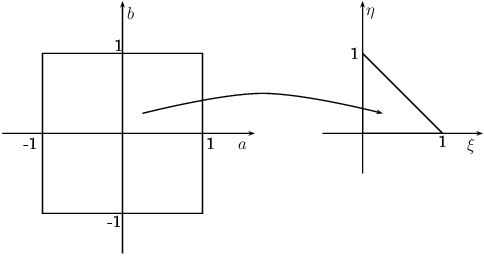
\includegraphics[width = 7cm]{./transformation.png}
    	\caption{Transformation between the reference square to the reference triangle}
    	\label{transformation}
    \end{center}
    \end{figure}
    
    The Dubiner basis is then constructed by a generalized tensor product of the Jacobi polynomials on the interval (-1, 1) to form a basis on the reference square, which is then transformed by the above “collapsing” mapping to a basis on the reference triangle.
    \begin{definition}[Jacobi polynomials]
    The Jacobi polynomials evaluated in $z\in \mathbb{R}^n$ are:
    \begin{itemize}[label=\textendash]
    \item $n=0$
    \begin{equation}
    J_0^{\alpha,\beta}(z)=\overbrace{\begin{bmatrix} 1 & 1 &\dots &1 \end{bmatrix}}^{\text{n times}}
    \end{equation}
    \item $n=1$
    \begin{equation}
    J_1^{\alpha,\beta}(z)=\frac{1}{2}(\alpha-\beta+(\alpha+\beta+2)\cdot z);
    \end{equation}
    \item $n\ge2$
    \newline
    \begin{equation}
    \begin{gathered}
    \begin{aligned}
    J_n^{\alpha,\beta}(z)=\sum_{k=2}^{n} \Big[&\frac{(2k+\alpha+\beta-1)(\alpha^{2}-\beta^{2})}{2k(k+\alpha+\beta)(2k+\alpha+\beta-2)}+ \\ &\frac{(2k+\alpha+\beta-2)(2k+\alpha+\beta-1)(2k+\alpha \beta)}{2k(k+\alpha+\beta)(2k+\alpha+\beta-2)} J_{k-1}^{\alpha,\beta}(z) +
    \\-&\frac{2(k+\alpha-1)(k+\beta-1)(2k+\alpha+\beta)}{2k(k+\alpha+\beta)(2k+\alpha+\beta-2)} J_{k-2}^{\alpha,\beta}(z) \Big]
    \end{aligned}
    \end{gathered}
    \end{equation}
    \end{itemize}
    \end{definition}
    
    An important property of this polynomials is:
    \begin{prop}
    $J_i^{\alpha,\beta}(\cdot)$ is orthogonal w.r.t. the Jacobi weight $w(x)=(1-x)^\alpha(1+x)^\beta$:
    \begin{equation}
    \int_{-1}^{1}{(1-x)^\alpha(1+x)^\beta J_m^{\alpha,\beta} J_q^{\alpha,\beta}(x)dx}=\frac{2}{2m+1} \delta_{mq} 
    \end{equation}
    \end{prop}
    
    Thanks to this definition, we can now look more accurately the formula of the Dubiner basis
    \begin{definition}[Dubiner Basis]
    \begin{equation}
    \begin{split}
    \phi_{ij}(\xi,\eta) :&= c_{ij}(1-b)^j J_i^{0,0}(a) J_j^{2i+1,0}(b)=
    \\&=c_{ij} 2^j (1-\eta)^j J_i^{0,0}(\frac{2\xi}{1-\eta}-1) J_j^{2i+1,0} (2\eta-1)
    \end{split}
    \end{equation}
    for $i,j=1,\dots,p$ and $i+j \le p$, where
    \begin{equation}
    c_{ij} := \sqrt{\frac{2(2i+1)(i+j+1)}{4^i}}
    \end{equation}
    and $J_i^{\alpha,\beta}(\cdot)$ is the i-th Jacobi polynomial
    \end{definition}
    
    We note that
    \begin{prop}
    $\phi_{ij}(\xi,\eta)$ is orthogonal w.r.t. Legendre internal product:
    \begin{equation}
    \iint_{\hat{K}}{\phi_{ij}(\xi,\eta)\phi_{mq}(\xi,\eta) d\xi d\eta}=\delta_{im}\delta_{jq}
    \end{equation}
    \end{prop}
    
    Indeed, we obtain a mass matrix diagonal as we can see in figure \ref{mass}
    
    \begin{figure}[ht]
    \begin{center}
    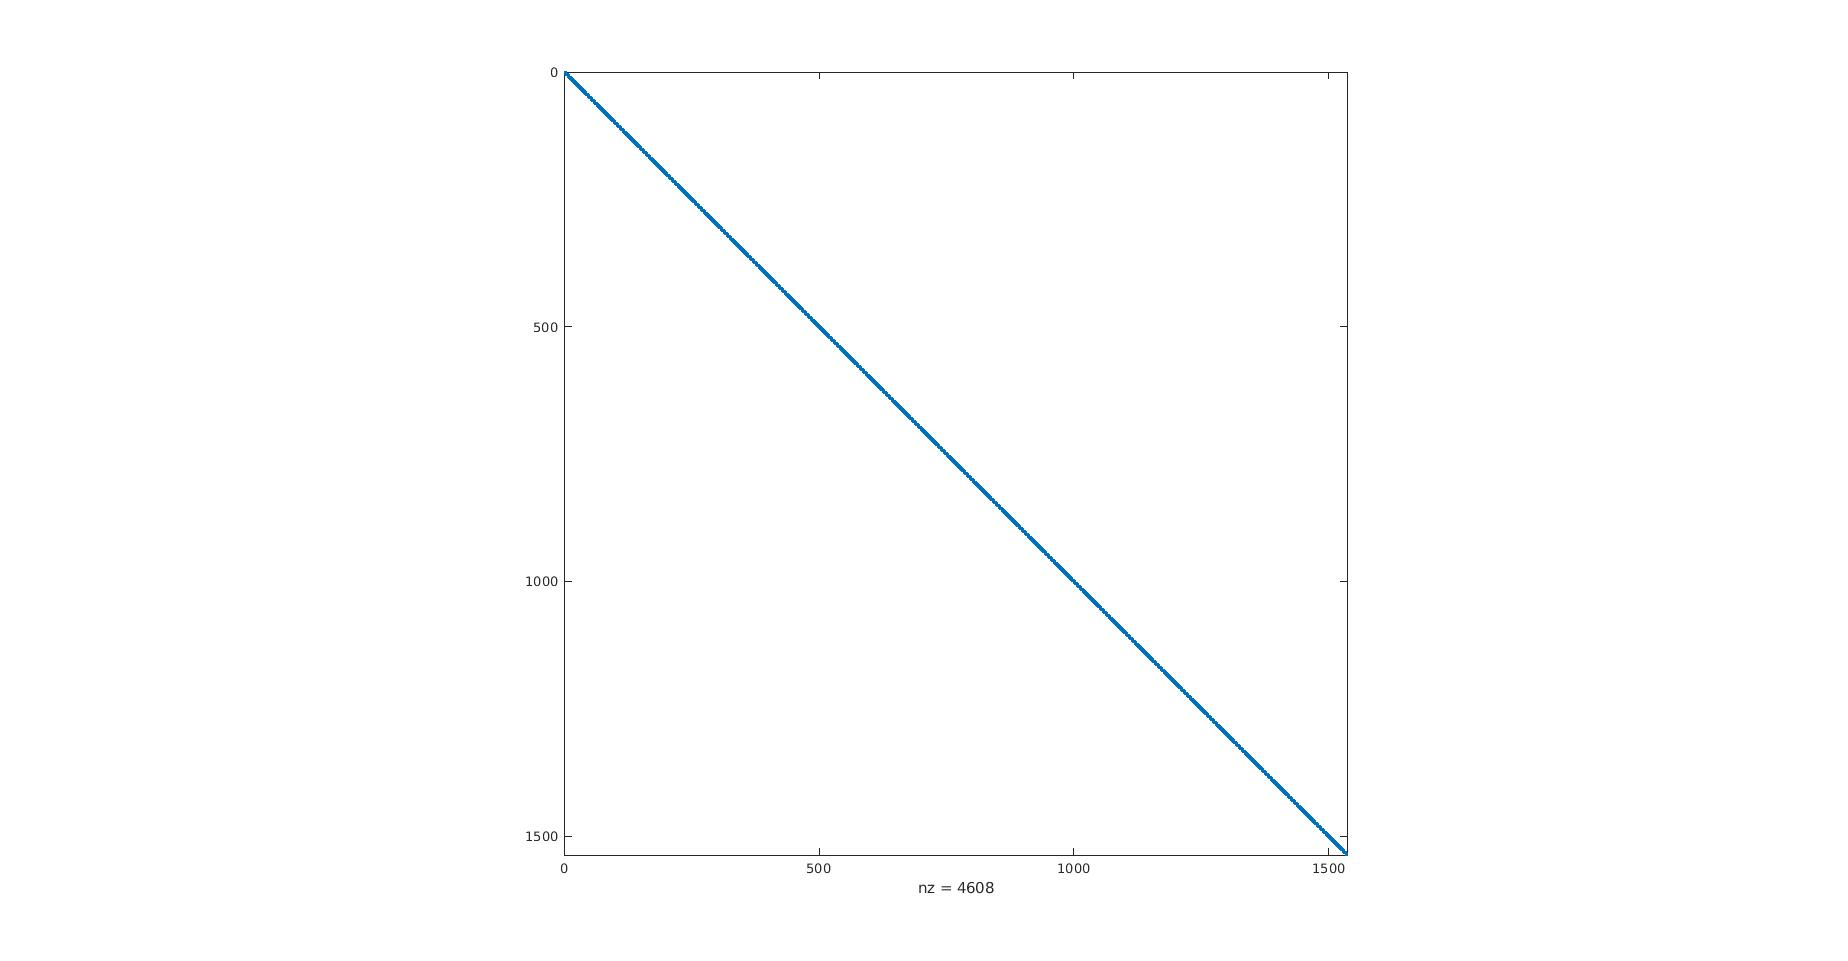
\includegraphics[width = 7cm]{./mass_dubiner.jpg}
    	\caption{Elements non zero in the mass matrix w.r.t Dubiner basis}
    	\label{mass}
    \end{center}
    \end{figure}
    
    \newpage
    \printbibliography

\end{document}

    
	
    
    
    
    
    
    
    
    
    
    
    
    \newpage
    \printbibliography

\end{document}
